\documentclass[14pt, fleqn, xcolor={dvipsnames, table}]{beamer}
\usepackage[T2A]{fontenc}
\usepackage[utf8]{inputenc}
\usepackage[english,russian]{babel}
\usepackage{amssymb,amsfonts,amsmath,mathtext}
\usepackage{cite,enumerate,float,indentfirst}
\usepackage{cancel}
\usepackage{graphicx}
\usepackage{animate}

\usepackage{tikz}
% \usepackage{enumitem}
\usetikzlibrary{shadows}

% \usepackage{enumitem}
% \setitemize{label=\usebeamerfont*{itemize item}%
%   \usebeamercolor[fg]{itemize item}
%   \usebeamertemplate{itemize item}}

\graphicspath{{images/}}

\usetheme{Madrid}
\usecolortheme{seahorse}
\renewcommand{\CancelColor}{\color{red}}

\setbeamercolor{footline}{fg=Blue!50}
\setbeamertemplate{footline}{
  \leavevmode%
  \hbox{%
  \begin{beamercolorbox}[wd=.333333\paperwidth,ht=2.25ex,dp=1ex,center]{}%
    И. Кураленок, Н. Поваров, Яндекс
  \end{beamercolorbox}%
  \begin{beamercolorbox}[wd=.333333\paperwidth,ht=2.25ex,dp=1ex,center]{}%
    Санкт-Петербург, 2014
  \end{beamercolorbox}%
  \begin{beamercolorbox}[wd=.333333\paperwidth,ht=2.25ex,dp=1ex,right]{}%
  Стр. \insertframenumber{} из \inserttotalframenumber \hspace*{2ex}
  \end{beamercolorbox}}%
  \vskip0pt%
}
\newcommand\indentdisplays[1]{%
     \everydisplay{\addtolength\displayindent{#1}%
     \addtolength\displaywidth{-#1}}}
\newcommand{\itemi}{\item[\checkmark]}

\newenvironment{mydescription}[1]
  {\begin{list}{}%
   {\renewcommand\makelabel[1]{\color{blue}##1:\hfill}%
   \settowidth\labelwidth{\makelabel{#1}}%
   \setlength\leftmargin{\labelwidth}
   \addtolength\leftmargin{\labelsep}}}
  {\end{list}}

\title{Обучение метрики\\\small{по Tutorial on Metric Learning by Brian Kulis}}
\author[]{\small{%
И.~Куралёнок,
Н.~Поваров}}
\date{}
\begin{document}

\begin{frame}
\maketitle
\small
\begin{center}
\vspace{-60pt}
\normalsize {\color{red}Я}ндекс \\
\vspace{80pt}
\footnotesize СПб, 2014
\end{center}
\end{frame}

\section{Содержание}
\section{Постановка проблемы}
\begin{frame}{Метрики в контексте IBL}
В прошлый раз использовали несколько buzzword, сегодня поговорим об одном из них --- дистанции между точками
\end{frame}

\begin{frame}{Пример с Михалычем}
Василий Петрович, хочет сталкиваться с Петром Михалычем чаще, причем желательно вдали от других рабочих завода.
\begin{description}
\item[Классы] разные люди
\item[Точки] появление в пространстве/времени человека $c$
\item[Действия] поговорить в громкоговоритель (одинаково повлиять на всех людей)
\end{description}
Надо помочь Петровичу правильно говорить в громкоговоритель.
\end{frame}

\begin{frame}{Как может выглядеть задача}
\begin{center}
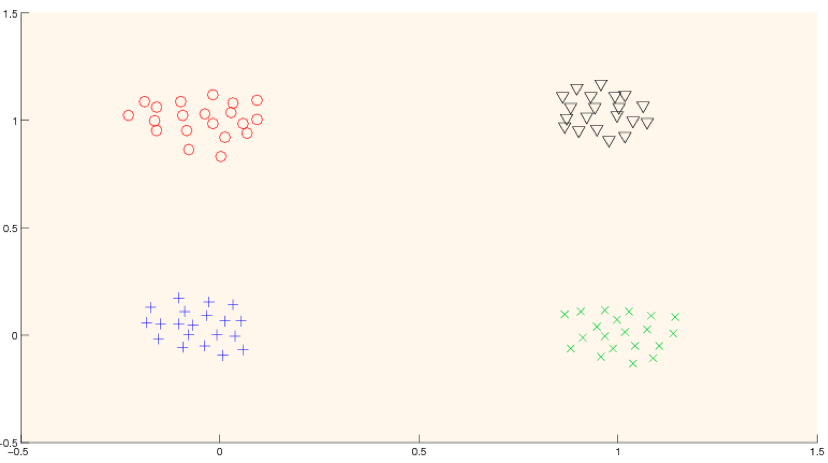
\includegraphics[width=0.9\textwidth]{linsep-setup.png}
\end{center}
\end{frame}

\begin{frame}{Как может выглядеть задача}
\begin{center}
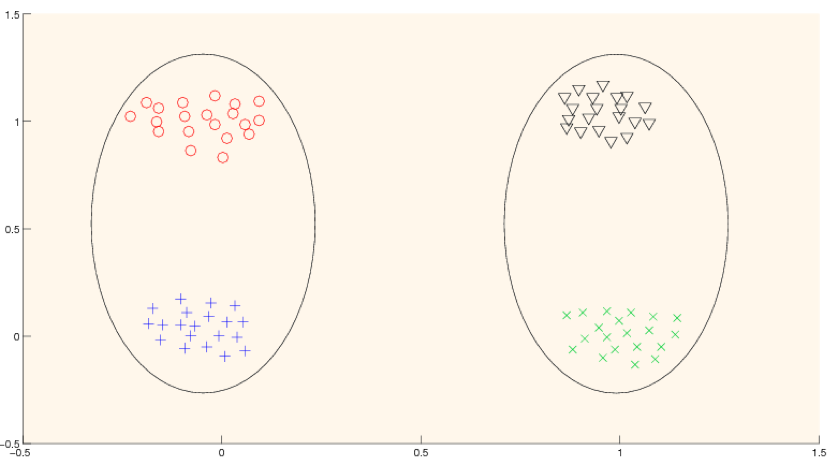
\includegraphics[width=0.9\textwidth]{linsep-setup2.png}
\end{center}
\end{frame}

\begin{frame}{Как может выглядеть решение}
\begin{center}
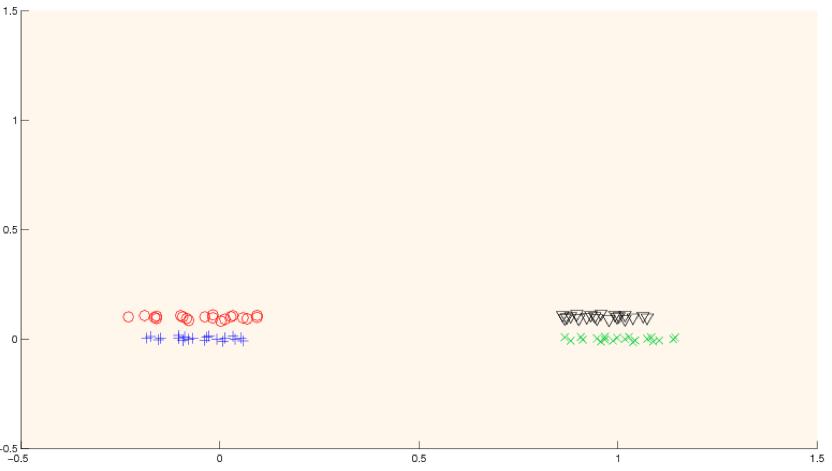
\includegraphics[width=0.9\textwidth]{linsep-solution.png}
\end{center}
\end{frame}

\begin{frame}{Как может выглядеть задача}
\begin{center}
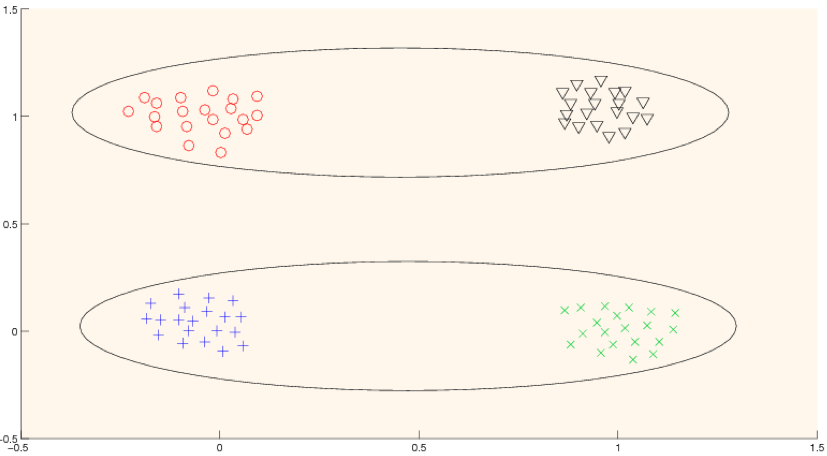
\includegraphics[width=0.9\textwidth]{linsep-setup3.png}
\end{center}
\end{frame}

\begin{frame}{Как может выглядеть решение}
\begin{center}
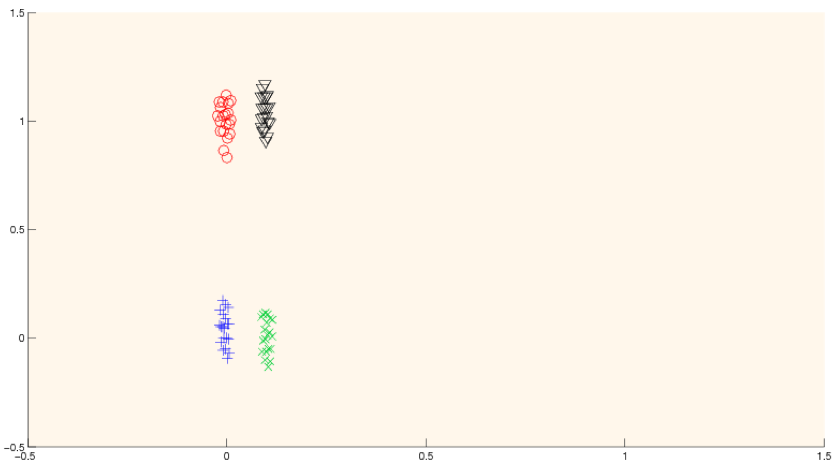
\includegraphics[width=0.9\textwidth]{linsep-solution2.png}
\end{center}
\end{frame}

\begin{frame}{Mahalanobis distance (постановка)}
\begin{description}
\item[Классы] нету
\item[Точки] какие-то точки, которых навалило
\item[Направления] одинаково значимые направления, померянные разной линейкой
\item[Действия] линейные преобразования пространства
\end{description}
$\Rightarrow$ хотим посчитать дистанцию, без учета линейки
\end{frame}

\begin{frame}{Mahalanobis distance (решение)}
\begin{itemize}
  \item $X = \{x_i | x_i \in \mathbb{R}^n\}$
  \item $\mu(a,b) = \|a - b\|_2^2$
\end{itemize}
$\Rightarrow$
$$\begin{array}{c}
\Sigma = \sum_{i,j} \left(x_i - \bar{x}\right)\left(x_j - \bar{x}\right)^T \\
\hat{\mu}(a,b) = \left(a - b\right) \Sigma^{-1} \left(a - b\right)
\end{array}$$
\end{frame}

\begin{frame}{Mahalanobis distance (решение)}
\begin{center}
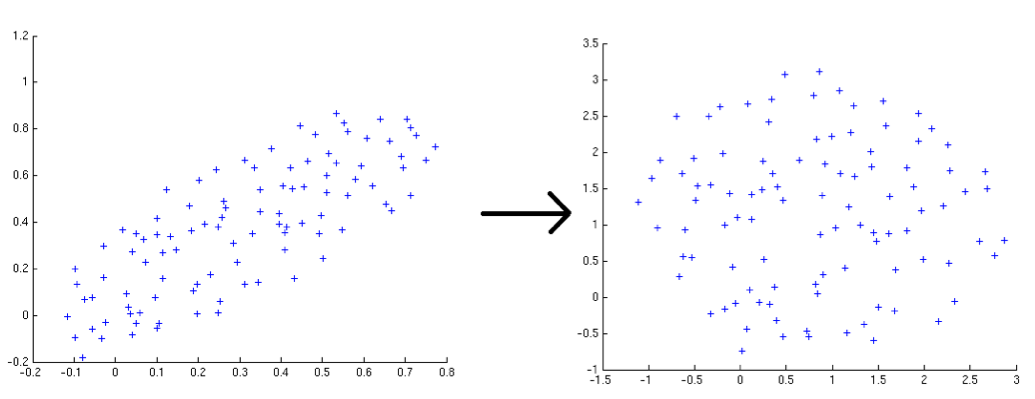
\includegraphics[width=0.9\textwidth]{mahalanobis.png}
\end{center}
\end{frame}

\begin{frame}{Постановка задачи обучения метрики}{}
{\color{blue}Дано:}
\begin{enumerate}
  \item Набор точек: $X = \{x_i | x_i \in \mathbb{R}^n\}$
  \item Исходная метрика $\mu_0(a,b)$ (например $\|a - b\|_q$, etc.)
  \item Условия группировки точек (классы/отношение расстояний/etc.): $T(X, \mu), \mu \in \mathcal{M}$
\end{enumerate}
{\color{blue}Найти:}\\
$$
\hat{\mu} = \arg \max_{\mu \in \mathcal{M}} T(X, \mu)
$$
\end{frame}

\section{Обучение линейного преобразования}

\begin{frame}{Постановка обучения Mahalanobis}{}
Будем искать решения в классе:
$$\begin{array}{ll}
\mathcal{M} = \{&\mu_A(a,b) | \\
& \mu_A(a,b) = (a - b)^T A (a - b), \\
& A \in PSD(\mathbb{R}^{n \times n})\\
\} &
\end{array}$$
\uncover<1>{Почему PSD?}\\
\uncover<2>{Если будет отрицательное собственное число, получится отрицательное значение метрики для собственного вектора}
\end{frame}

\begin{frame}{Немного о метриках}{}
\small
Метрика это такое преобразование $\mu : X^2 \to \mathbb{R}$:
\begin{enumerate}
  \item $\mu(a,b) \ge 0$
  \item $\mu(a,b) = 0 \Leftrightarrow a = b$
  \item $\mu(a,b) = \mu(b,a)$
  \item $\mu(a,c) \le \mu(a,b) + \mu(b,c)$
\end{enumerate}
$\mu_A$ --- не метрика. Метрикой является $\mu^{*} = \sqrt{\mu_A}$ в случае, когда $A \succ 0$. Такое добро зовется ``псевдометрика''.
\end{frame}

\begin{frame}{Вспоминая исходный пример}
\begin{center}
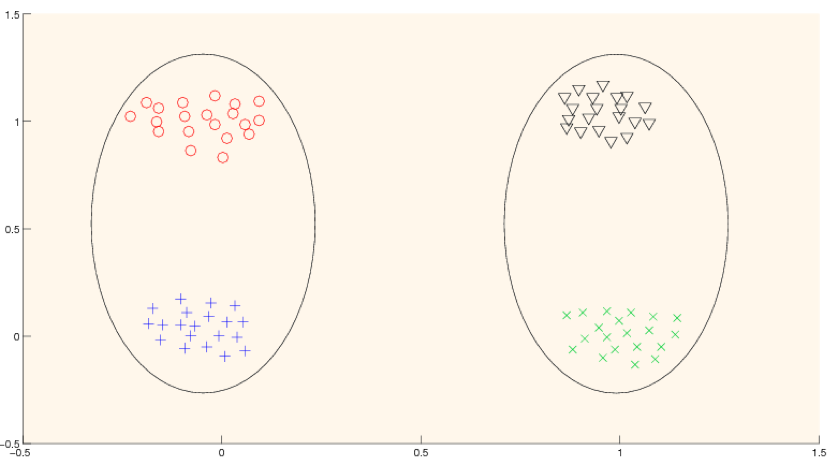
\includegraphics[width=0.9\textwidth]{linsep-setup2.png}
\end{center}
\end{frame}

\begin{frame}{Как может выглядеть решение}
\begin{center}
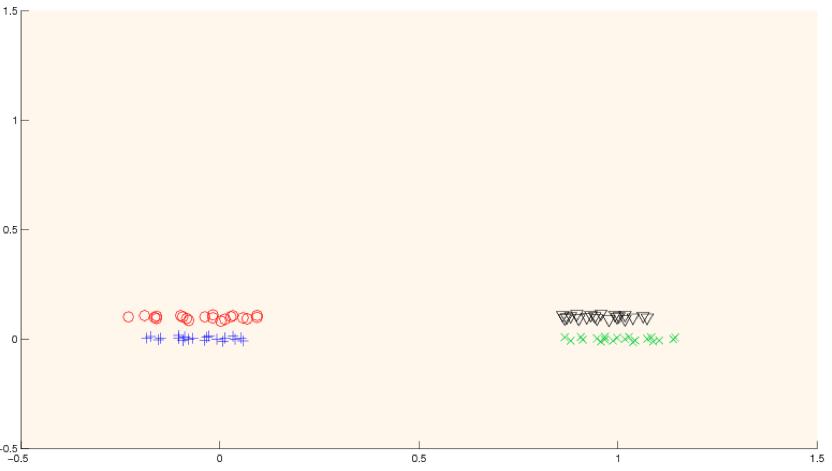
\includegraphics[width=0.9\textwidth]{linsep-solution.png}
\end{center}
$$
A = \left(\begin{array}{cc}
1 & 0 \\
0 & \epsilon
\end{array}\right)
$$
\end{frame}

\begin{frame}{Свойства Mahalanobis метрик}
\begin{itemize}
  \item Надо хранить матрицу $A$, которая большая и в общем случае dense
  \item Работает только в случае линейной разделимости ``разных'' примеров
\end{itemize}
\begin{center}
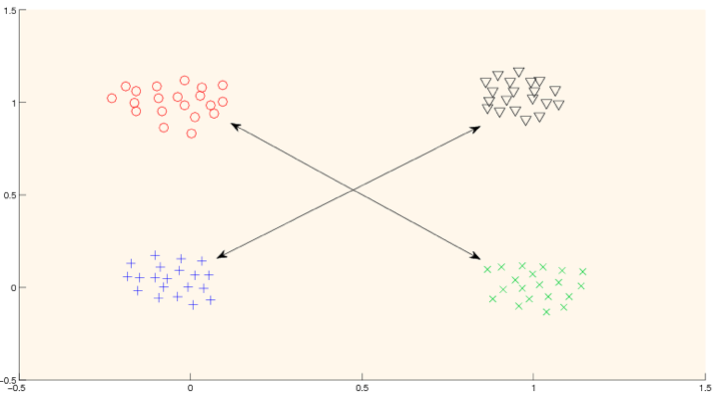
\includegraphics[width=0.7\textwidth]{linnonsep.png}
\end{center}
\end{frame}

\begin{frame}{Варианты целевой функции}
\small
Желания по тому какими свойствами должна обладать метрика можно выражать по-разному:\\
{\color{blue}Условия группировки}\\
\footnotesize
\begin{itemize}
     \item Есть два множества $\mathcal{S}, \mathcal{D} \subset X^2$ точек, которые должны быть поближе/подальше
     \item $(a,b) \in \mathcal{S} \Leftrightarrow \mu_A(a,b) \le l$,  $(a,b) \in \mathcal{D} \Leftrightarrow \mu_A(a,b) \ge u$
\end{itemize} 
{\small\color{blue}Условия относительной близости}\\
\footnotesize
\begin{itemize}
     \item Зададим такое множество троек $\mathcal{K} \subset X^3$, в котором первая точка должна быть поближе ко второй чем к третьей
     \item $(a,b,c) \in \mathcal{K} \Leftrightarrow \mu_A(a,b) \le \mu_A(a,c) - m$
\end{itemize} 
\small
Оба эти случая мы можем аггрегировать простым суммированием введя расслабляющие коэффициенты
\end{frame}

\begin{frame}{Варианты регуляризации}
Нас могут устраивать больше одни варианты $A$ нежели другие, мы можем выразить это регуляризацией:
\begin{itemize}
  \item Отклонение по Фробениусу от какой-то хорошей матрицы (например от прошлого оптимума):
  $$
  \|A - A_0\|_F^2
  $$
  \item LogDet divergence от хорошей матрицы: $D_{ld}(A,A_0) = tr(AA_0^{-1}) - \log \det(AA_0^{-1}) - d$
  \item Простая фробениус норма $\|A\|_F$ --- аналог $l_2$
  \item $tr(AC_0)$ --- аналог $l_1$
\end{itemize}
\end{frame}

\begin{frame}{Немного про LogDetDiv}
\footnotesize
Используется в основном в картинках. Пусть $X = V \Lambda V^T$, а $Y = U \Theta U^T$, тогда:
$$\begin{array}{rl}
D_{ld}(X,Y) &= tr(XY^{-1}) - \log \det(XY^{-1}) - d \\
&= tr(Y^{-\frac{1}{2}}XY^{-\frac{1}{2}})  - \log \det (Y^{-\frac{1}{2}}XY^{-\frac{1}{2}}) - d \\
&= tr(Y^{-\frac{1}{2}}XY^{-\frac{1}{2}} - \log Y^{-\frac{1}{2}}XY^{-\frac{1}{2}} - E) \\
&= \sum_i\sum_j(v^T_i, u_j)^2\left(\frac{\lambda_i}{\theta_j} - \log(\frac{\lambda_i}{\theta_j}) - 1\right)
\end{array}$$
Обладает такими свойствами:
\begin{itemize}
\item Инвариантна к линейному обратимому преобразованию
\item 0 только при равенстве, иначе позитивна
\item Pythagorean условие на выпуклых множествах $\Omega$ (упрощенный треугольник)
\item Несимметрична
\item Можно расширить на полуопределенные матрицы
\end{itemize}
\end{frame}

\begin{frame}{MMC}
$$\begin{array}{l}
max_A \sum_{(a, b) \in \mathcal{D}} \sqrt{\mu_A(a, b)} \\
c(A) = \sum_{(a, b) \in \mathcal{S}} \mu_A(a, b) \le 1 \\
A \succeq 0
\end{array}$$

\begin{itemize}
  \item $\mathcal{D}$ это множество различающихся, а $\mathcal{S}$ - множество одинаковых
  \item Пытаемся максимизировать сумму расстояний для различающихся
  \item Хотим маленькую сумму расстояний одинаковых
\end{itemize}
\end{frame}


\begin{frame}{MMC: алгоритм}
\begin{itemize}
  \item Градиентный спуск сопровождается поиском подходящей $A$
  \begin{itemize}
    \item Ограничение $c(A)$ линейно по $A$, а значит разрешается дёшево
  \end{itemize}
  \item Несмотря на относительную простоту, алгоритм медленный
  \item Не масштабируется
\end{itemize}
\end{frame}


\begin{frame}{Schultz and Joachims}
$$\begin{array}{l}
min_A \|A\|_{F}^2 \\
\mu_A(x_i, x_k) - \mu_{A}(x_i, x_j) \ge 1 \;\;\;\; \forall (x_i,x_j,x_k) \in \mathcal{K} \\
A \succeq 0
\end{array}$$
В такой формулировке может не иметь решения, тогда

$$\begin{array}{l}
min_{A, \xi} \|A\|_{F}^2 + \gamma \sum_{(i,j,k) \in \mathcal{R}} \xi_{ijk} \\
\mu_A(x_i, x_k) - \mu_{A}(x_i, x_j) \ge 1 - \xi_{ijk} \;\;\;\; \forall (x_i,x_j,x_k) \in \mathcal{K} \\
\xi_{ijk} \ge 0 \;\;\; \forall (i,j,k) \in \mathcal{R} \\
A \succeq 0
\end{array}$$

\end{frame}

\begin{frame}{Schultz and Joachims: Алгоритм}
\begin{itemize}
  \item Главное упрощение:
  \begin{itemize}
    \item $A = M^TDM$, где $М$ фиксировано и известно, а $D$ - диагональная
    $$\begin{array}{rl}
      \mu_A(x_i, x_j) &= (x_i - x_j)^TA(x_ - x_j) \\
      &= (x_i - x_j)^TM^TDM(x_ - x_j) \\
      &= (Mx_i - Mx_j)^TD(Mx_ - Mx_j) \\
\end{array}$$
    \item Итоговая оптимизационная проблема очень похожа на SVM

  \end{itemize}
  \item С помощью $M$ метод можно кернелизировать
  \item Алгоритм быстрый, но менее общий, чем Mahalanobis
\end{itemize}
\end{frame}

\begin{frame}{Neighbourhood Components Analysis}
$$
\max_{A \succeq 0} \sum_{(i,j)\in\mathcal{S}} {e^{-\mu_A(x_i,x_j)} \over \sum_{k\ne i} e^{-\mu_A(x_i, x_k)}}
$$
Минимизируем LOO kNN классификатор:
\small
\begin{itemize}
  \item если честный LOO, то получим прерывную функцию;
  \item вместо значения 0/1 из ближайшего соседа, переписываем в soft max моделируя вероятность так:
  $$
  p_{ij} = {e^{-\mu_A(x_i,x_j)} \over \sum_{k\ne i} e^{-\mu_A(x_i, x_k)}}
  $$
\end{itemize}
\end{frame}

\begin{frame}{Neighbourhood Components Analysis}{Алгоритм и свойства}
Оптимизация:
\begin{itemize}
  \item Проблема невыпукла
  \item Переписываем $A = G^TG$, чтобы не думать про $A \succeq 0$
  \item Градиентный спуск по компонентам $G$
\end{itemize}
Свойства:
\begin{itemize}
  \item Легко контролировать ранк $A$, контролируя ранк $G$
  \item Простая безусловная оптимизация
  \item Без гарантий глобальной сходимости
\end{itemize}
\end{frame}

\begin{frame}{Онлайн постановка, POLA}
Часто данные приходят последовательно. Попробуем строить $\mu_A$ последовательно:
\begin{itemize}
  \item На каждом шагу наблюдаем тройку: $(a_t,b_t,y_t)$, если $y_t = 1$, то хотим точки поближе, если $y_t = -1$ --- сделаем подальше.
  \item Будем оптимизировать такой loss \uncover<2>{(hinge loss)}
  $$
  l(A, y) = \max(0, y_t(\mu_A(a_t,b_t) - b) + 1)
  $$
  \item Оптимизировать будем (как и в любой online постановке):
  $$
  R_T = \sum_{t=1}^{T} l_t(A^*, b^*) - \sum_{t=1}^{T} l_t(A_t, b_t) 
  $$
\end{itemize}
\end{frame}

\begin{frame}{POLA: алгоритм}
\begin{enumerate}
  \item Введем 2 выпуклых множества:
  $$\begin{array}{c}
  C_t = \{(A,b) | l_t(A,b) = 0\} \\
  C_A = \{(A,b) | A \succeq 0 b > 0\}
  \end{array}$$
  \item Научимся проецировать на эти множетсва (есть идеи как?)
  \item На каждом шагу будем сначала проэцировать на новый $C_t$, а потом на $C_A$ 
\end{enumerate}
\end{frame}


\begin{frame}{ITML как пример LogDet}
Так долго говорили про LogDet, надо бы где-нибудь поиспользовать :).
$$\begin{array}{l}
\min_{K\in PSD(\mathbb{R}^{m\times m})} T(K,K_0) \\
\left\{\begin{array}{l}
(a - b)^T A (a - b) \le u, \forall (a,b) \in \mathcal{S} \\
(a - b)^T A (a - b) \ge l, \forall (a,b) \in \mathcal{D} \\
\end{array}\right.
\end{array}$$
Там много математики, но смысл в том, что можно свести к такому построению матрицы:
$$A_{t+1} = A_t + \beta_t A_t (x_i - x_j)(x_i - x_j)^TA_t$$
\end{frame}

\begin{frame}{Не-Махаланобисовы методы: LDF}{Local distance functions}
\small
Хотим сделать громкоговоритель локальнее: в столовой --- один, в цеху --- другой.
Для этого пожертвуем сложностью модели, забыв о зависимости по осям:
$$
\mu(a,b) = \sum_m w_a(m) d(a_{m}, b_{m})
$$
Заметим, что несмотря на несимметричность модели, мы все же можем построить kNN. \\
$\Rightarrow$ можно поставить задачу совместной оптимизации $w$. Например так:
$$\begin{array}{l}
\min_{w} \sum_i \|w_i\|_q \\
\mu(a, b) - \mu(a, c) \ge 1, \forall (a, b, c) \in \mathcal{K} \\
w_i\ge 0, \forall i
\end{array}$$
\footnotesize Сравните постановку с Schultz and Joachims
\end{frame}

\section{Кернелизация}
\begin{frame}{Проблема линейной неразделимости}
Где-то мы это уже видели, сделаем ядро!
\begin{center}
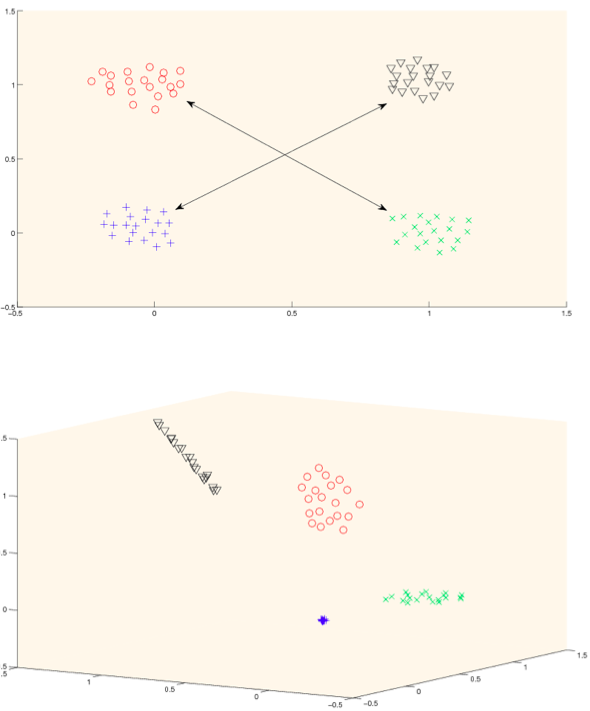
\includegraphics[height=0.7\textheight]{kernel.png}
\end{center}
\end{frame}

\begin{frame}{Кернелизация ITML}
Вспомним шаг алгоритма:
$$A_{t+1} = A_t + \beta_t A_t (x_i - x_j)(x_i - x_j)^TA_t$$
Домножим слева/справа на матрицу $X$ и раскроем скобки в терминах новых скалярных произведений ($x^TAy$):
$$X^TA_{t+1}X = X^TA_tX + \beta_t X^T A_tX(e_i - e_j)(e_i - e_j)^TX^TA_tX$$
Тогда в терминах ядер ($k^t_{ij} = x_i^T A_t x_j$):
$$K^{t+1} = K^{t} \beta_t K^{t} (e_i - e_j)(e_i - e_j)^T K^{t}$$
Также можно делать и с другими алгоритмами, которые мы сегодня рассмотрели
\end{frame}

\begin{frame}{Постановка kernel learning для metric learning}
\small
Давайте ограничемся только квадратом евклидовой метрики (уже в kernel space):
$$\|a - b\|_2^2 = x_i^Tx_i + x_j^T x_j - 2 x_i^T x_j$$
Что можно переписать в терминах ядер:
$$k_{ii} + k_{jj} - 2 k_{ij}$$
Будем считать, что условия у нас заданы в терминах группировки. Тогда оптимизацию можно переписать:
$$\begin{array}{l}
\min_{K\in PSD(\mathbb{R}^{m\times m})} T(K,K_0) \\
\left\{\begin{array}{l}
k_{ii} + k_{jj} - 2 k_{ij} \le u, \forall (i,j) \in \mathcal{S} \\
k_{ii} + k_{jj} - 2 k_{ij} \ge l, \forall (i,j) \in \mathcal{D} \\
\end{array}\right.
\end{array}$$
\end{frame}

\section{Заключение}
\begin{frame}{Что мы сегодня узнали}
\begin{itemize}
  \item Расстояние можно менять
  \item Удобно работать с неметриками, убрав правило треугольника
  \item Точно как поставить задачу обучения метрики
  \item Есть несколько способов обучить линейное преобразование, в том числе online
  \item Сообщество любителей ядер постаралось и на этой ниве, что позволяет решать линейно неразделимые задачи
\end{itemize}
\end{frame}
\end{document}
